\section{Method} \label{section:method}

The intuition behind the \acrshort{tqn}, shared by the related work on offline \acrshort{rl} \cite{decision_transformer,q_transformer}, is that a set of observations, on which the network is trained, can be seen as a sequence, for which the Transformer architecture is particularly suited.

By replacing the first layer of a \acrshort{dqn} with a Transformer layer, the neural network can extract more relevant features, and the multi-head attention mechanism is trained to recognize the more relevant observations from the set, without the added complexity of a \acrshort{per}. However, this happens on a smaller scale, since \acrshort{per} samples the most important experiences from the entire experience replay, while the multi-head attention chooses the most relevant experiences from a smaller set of observations.

The expected result can become a viable way to increase stability during training and to improve performance, leading to a quicker convergence to the optimal policy.

\subsection{Baseline}
The input to the neural network consists of a tensor containing the state of the environment. The neural network processes the input through  two hidden layers consisting of $256$ units, both followed by a rectifier nonlinearity. The output layer is a linear layer whose values are the predicted Q-values for each individual action, given the input state \cite{dqn1,dqn2}. Each layer of the neural network is a fully-connected layer (see \textbf{Fig.}~\ref{fig:dqn-architecture}. In order to reduce over-estimation, a copy of the network is used to evaluate the predictions (see \nameref{subsubsec:double_dqn}).

\begin{figure}[!htbp]
\tikzset{
  every neuron/.style={
    circle,
    draw,
    minimum size=1cm
  },
  neuron missing/.style={
    draw=none, 
    scale=4,
    text height=0.333cm,
    execute at begin node=\color{black}$\vdots$
  },
}
\centering
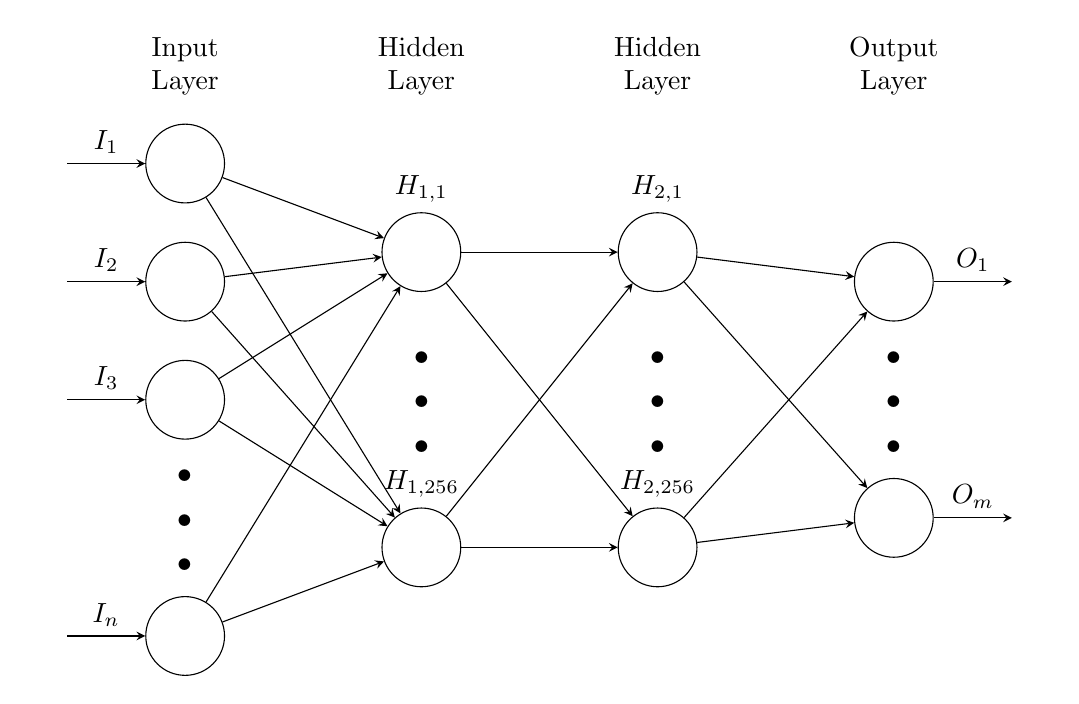
\begin{tikzpicture}[x=1.5cm, y=1.5cm, >=stealth]

\foreach \m/\l [count=\y] in {1,2,3,missing,4}
  \node [every neuron/.try, neuron \m/.try] (input-\m) at (0,2.5-\y) {};

\foreach \m [count=\y] in {1,missing,2}
  \node [every neuron/.try, neuron \m/.try ] (hidden1-\m) at (2,2-\y*1.25) {};

\foreach \m [count=\y] in {1,missing,2}
  \node [every neuron/.try, neuron \m/.try ] (hidden2-\m) at (4,2-\y*1.25) {};

\foreach \m [count=\y] in {1,missing,2}
  \node [every neuron/.try, neuron \m/.try ] (output-\m) at (6,1.5-\y) {};

\foreach \l [count=\i] in {1,2,3,n}
  \draw [<-] (input-\i) -- ++(-1,0)
    node [above, midway] {$I_\l$};

\foreach \l [count=\i] in {1,256}
  \node [above] at (hidden1-\i.north) {$H_{1,\l}$};

\foreach \l [count=\i] in {1,256}
  \node [above] at (hidden2-\i.north) {$H_{2,\l}$};

\foreach \l [count=\i] in {1,m}
  \draw [->] (output-\i) -- ++(1,0)
    node [above, midway] {$O_\l$};

\foreach \i in {1,...,4}
  \foreach \j in {1,...,2}
    \draw [->] (input-\i) -- (hidden1-\j);

\foreach \i in {1,...,2}
  \foreach \j in {1,...,2}
    \draw [->] (hidden1-\i) -- (hidden2-\j);

\foreach \i in {1,...,2}
  \foreach \j in {1,...,2}
    \draw [->] (hidden2-\i) -- (output-\j);

\foreach \l [count=\x from 0] in {Input, Hidden, Hidden, Output}
  \node [align=center, above] at (\x*2,2) {\l \\ Layer};

\end{tikzpicture}
\caption{The \acrlong{dqn} architecture.}
\label{fig:dqn-architecture}
\end{figure}

\subsection{Transformer Q-Network}

The Transformer Q-Network consists instead of an encoding component, a decoding component, followed by two hidden fully-connected layers and the output layer. Both the encoding and decoding components also stack two hidden layers each, all sharing the same parameters. Each encoder/decoder layer has an input and output size equal to the observation size, with a hidden layer of size $256$. The dropout value is set to $0.1$ and the attention heads are set equal to the observation size, which can be  $4$, $6$ or $8$ depending on the environment.


\begin{figure}[H] 
\centering
\subfloat{%
\resizebox{0.35\textwidth}{!}{
\tikzset{
  every neuron/.style={
    circle,
    draw,
    minimum size=1cm
  },
  neuron missing/.style={
    draw=none, 
    scale=4,
    text width=0.333cm,
    execute at begin node=\color{black}$\ldots$
  },
}
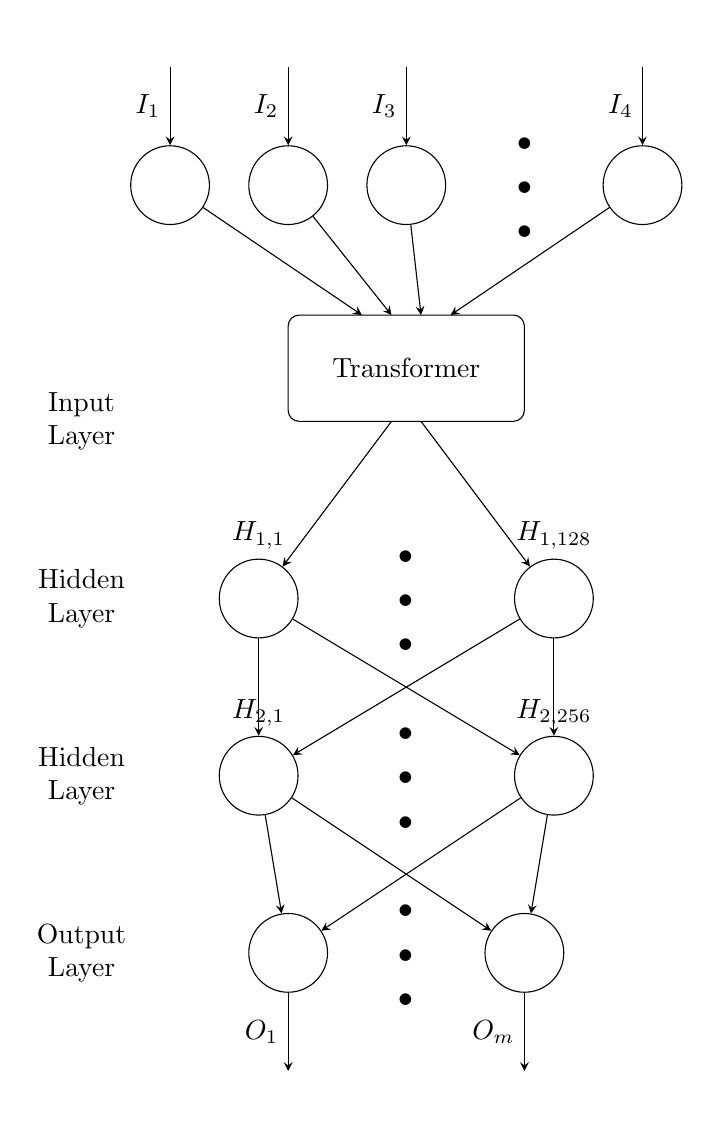
\begin{tikzpicture}[x=1.5cm, y=1.5cm, >=stealth]%
  
\foreach \m/\l [count=\x] in {4,missing,3,2,1}
  \node [every neuron/.try, neuron \m/.try] (input-\m) at (0.25-\x, 6.5) {};

\draw [rounded corners] (-3.75,4.5) rectangle (-1.75,5.4);
\node [anchor=center] at (-2.75,4.95) {Transformer};

\foreach \m [count=\x] in {1,missing,2}
  \node [every neuron/.try, neuron \m/.try ] (hidden1-\m) at (-0.25-\x*1.25,3) {};

\foreach \m [count=\x] in {1,missing,2}
  \node [every neuron/.try, neuron \m/.try ] (hidden2-\m) at (-0.25-\x*1.25,1.5) {};

\foreach \m [count=\x] in {1,missing,2}
  \node [every neuron/.try, neuron \m/.try ] (output-\m) at (-0.75-\x,0) {};

\foreach \l [count=\i] in {1,2,3,4}
  \draw [<-] (input-\i) -- ++(0,1)
    node [midway, left] {$I_\l$};

\foreach \l [count=\i] in {128, 1}
  \node [above] at (hidden1-\i.north) {$H_{1,\l}$};

\foreach \l [count=\i] in {256, 1}
  \node [above] at (hidden2-\i.north) {$H_{2,\l}$};

\foreach \l [count=\i] in {m,1}
  \draw [->] (output-\i) -- ++(0,-1)
    node [midway, left] {$O_\l$};

\foreach \i in {1,...,4}
    \draw [->] (input-\i) -- (-3.375 + 0.25*\i,5.4);

\def\hiddenlist{{2,1}}
\foreach \i [evaluate=\i as \y using {\hiddenlist[\i-1]}] in {1,...,2} {
    \draw [->] (-3.125 + 0.25*\i,4.5) -- (hidden1-\y);
}

\foreach \i in {1,...,2}
  \foreach \j in {1,...,2}
    \draw [->] (hidden1-\i) -- (hidden2-\j);

\foreach \i in {1,...,2}
  \foreach \j in {1,...,2}
    \draw [->] (hidden2-\i) -- (output-\j);

\foreach \l [count=\y from 0] in {Output, Hidden, Hidden, Input}
  \node [align=center] at (-5.5,\y*1.5) {\l \\ Layer};

\end{tikzpicture}%
}%
}%
\hfill%
\subfloat{%
\raisebox{1.5cm}[0pt][0pt]{%
\makebox[0.64\textwidth][c]{\includegraphics[width=0.64\textwidth]{images/exploded-encoder-decoder.png}}%
}%
}%
\caption[On the left, a simplified view of the \acrlong{tqn}. On the right, the inner components of the Transformer layer. Image on the right adapted from ``The Illustrated Transformer".]{On the left, a simplified view of the \acrlong{tqn}. On the right, the inner components of the Transformer layer. Image on the right adapted from ``The Illustrated Transformer"\protect\footnotemark.}
\label{fig:tqn-architecture}
\end{figure}

\footnotetext{\url{https://jalammar.github.io/illustrated-transformer/}}


First, the batch of observations gets reshaped to a single batch, containing a sequence of observations, the previous batch size is now the length of the sequence. The encoder/decoder pair extracts the relevant features from the observation, then the two fully-connected hidden layers of size $128$ and $256$, respectively, process it further. Each linear layer is always followed by a rectifier nonlinearity activation function. Finally, the output layer is again a linear layer whose values are the predicted Q-values for each possible action.


\subsection{A Note on Embedding}
Embedding is used with the attention model to transform a discrete token of the input sequence in a continuous vector representation. For the chosen environments, the observation is already in the form of a vector of floating point numbers, therefore preprocessing it through an embedding layer is not needed.

Depending on the task, before embedding a sequence, each token may be augmented with positional encoding. Again, this step was deemed not needed for two reasons: the sequence is not going through an embedding layer, and each observation does not temporally come after the previous one, but it is independently sampled from the experience replay. Preliminary iterations of the network that also employed an embedding step had the score over time collapse towards the worst possible value with no sign of recovery.

\begin{algorithm}
\caption{\textbf{Baseline}: Double DQN with Experience Replay \cite{dqn1,dqn2,double_dqn}}
\label{alg:baseline}
\begin{algorithmic}
\State Initialize replay memory $\mathcal{D}$ to capacity $N$
\State Initialize action-value function $Q$ with random weights
\For {episode $ = 1, M$}
\State Initialize sequence $s_1 = \{ x_1 \}$
\For {$t = 1, T$}
\State With probability $\epsilon$ select a random action $a_t$
\State otherwise select $a_t = \max_a Q^*(s_t, a; \theta)$
\State Set $s_{t+1} = s_t, a_t, x_{t+1}$
\State Store transition $(s_t, a_t, r_t, s_{t+1})$ in $\mathcal{D}$
\State Sample random minibatch of transitions $(s_j, a_j, r_j, s_{j+1})$ from $\mathcal{D}$
\State Set $ y_j =
\begin{cases}
r_j &\text{for terminal } s_{j+1} \\
r_{j+1} + \gamma Q(s_{t+1}, \argmax_{a} Q(s_{j+1}, a; \theta); \theta_{\text{target}}) &\text{for non-terminal } s_{j+1}
\end{cases}
$
\State Perform a gradient descent step on $(y_j - Q(s_j, a_j; \theta))^2$
\EndFor
\EndFor
\end{algorithmic}
\end{algorithm}
